\documentclass[11pt,spanish]{article}
\usepackage[spanish]{babel}
\selectlanguage{spanish}
\usepackage[utf8]{inputenc}
\DeclareUnicodeCharacter{2212}{-}
\DeclareUnicodeCharacter{2265}{+}
\usepackage{graphicx}
\usepackage{mathtools}
\usepackage{amssymb}
\usepackage{xcolor}
\usepackage{float}
\usepackage{hyperref}
\usepackage{subfigure}
\usepackage{blindtext}
\usepackage{geometry}
 \geometry{
 a4paper,
 total={170mm,257mm},
 left=20mm,
 top=20mm,
 }




\begin{document}

\begin{titlepage}
	\centering
	
\includegraphics[width=0.15\textwidth]{Emblema_Universidad_de_Sevilla.png}\par\vspace{1cm}
	{\scshape\LARGE Universidad de Sevilla \par}
	\vspace{1cm}
	{\scshape\Large Trabajo de programación\par}
	\vspace{1.5cm}
	{\huge\bfseries Spotify\par}
	\vspace{2cm}
	{\Large\itshape Abraham Corta Ramírez y José Calcedo Vázquez\par}
	\vfill
	
	{\large \today\par}
\end{titlepage}


\pagenumbering{gobble}

\newpage
\pagenumbering{arabic}

\tableofcontents

\listoffigures

\clearpage

\section{Introducción a Spotify}

\paragraph*{Para este trabajo de programación la plataforma que vamos a utilizar es Spotify, esta aplicación es empleada para la reproducción de música vía streaming. Actualmente Spotify es uno de los líderes del sector y contiene millones de canciones y cientos de miles de artistas de todos los géneros.}

\paragraph*{Spotify ofrece una \href{https://developer.spotify.com/documentation/web-api/}{Web API} con la que nos permite acceder a numerosos datos como canciones, artistas, playlists, etc. Y no solo eso, sino que de una canción en concreto se pueden obtener datos como su tempo, la duración, su grado de «instrumentalidad», de energía, etc. Esta API se puede utilizar con diferentes lenguajes como PHP, Java, JavaScript o Python entre otras mediante el uso de librerías.}

\paragraph*{Nosotros hemos decido hacerlo con Python debido a que es mas ligero que Java y más simple de utilizar.}

\paragraph*{La API se compone de muchos componentes, a continuación, se nombran algunos de estos:}

\begin{itemize}
	\item \textbf{Peticiones}
	\item \textbf{Spotify URls e IDs }
	\item \textbf{Respuestas: en formato JSON}
	\item \textbf{Paginación}
	\item \textbf{Autenticación }
\end{itemize}

\paragraph*{Nuestro objetivo será manipular los datos de la API sobre un artista en concreto, y partiendo de ahí estudiaremos sus conexiones, los artistas relacionados y las playlists.}

\paragraph*{El primer paso es crearnos \href{https://developer.spotify.com/dashboard/applications}{una cuenta como desarrollador Spotify}, 
	si ya tenemos cuenta de Spotify solo necesitaremos iniciar sesión en la web de desarrolladores. Será necesario dar de alta una aplicación [Figura~\ref{fig:dashboard_spotify}], de esta manera obtendremos un Client ID y un Client Secret [Figura~\ref{fig:app_spotify}].
	\footnote{Se han ocultado los client ID de las figuras ya que este puede ser usado por cualquier persona.}}

\begin{figure}[h!]
    \centering
    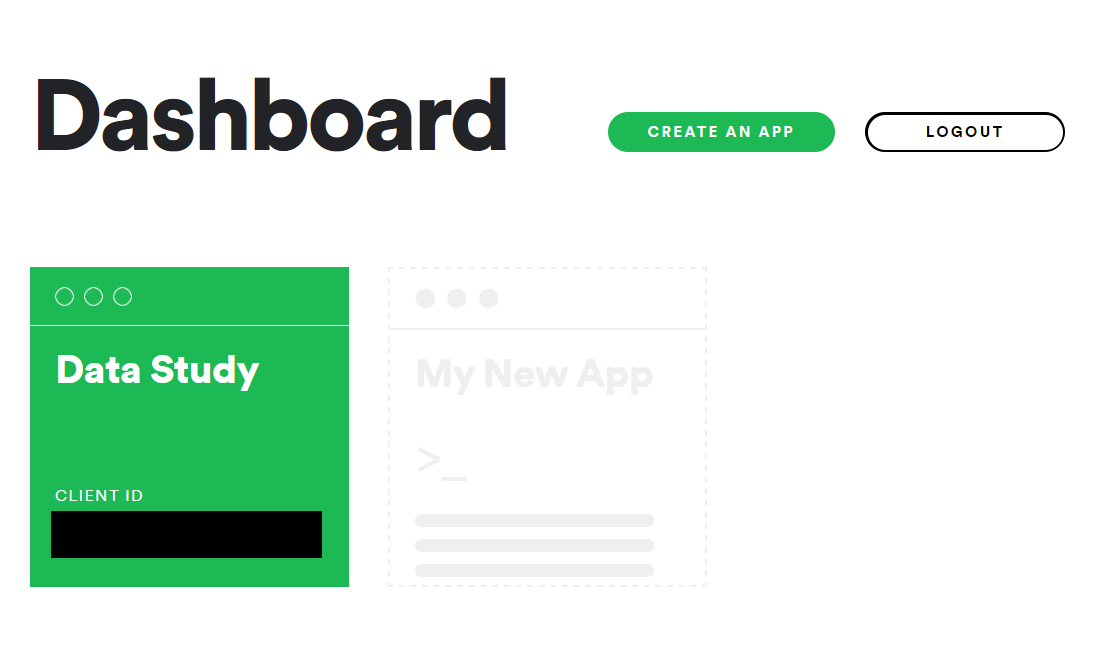
\includegraphics[width=120mm]{spotify_dev_dashboard.png}
    \caption{Spotify dashboard}\label{fig:dashboard_spotify}
\end{figure}

\begin{figure}[h!]
    \centering
	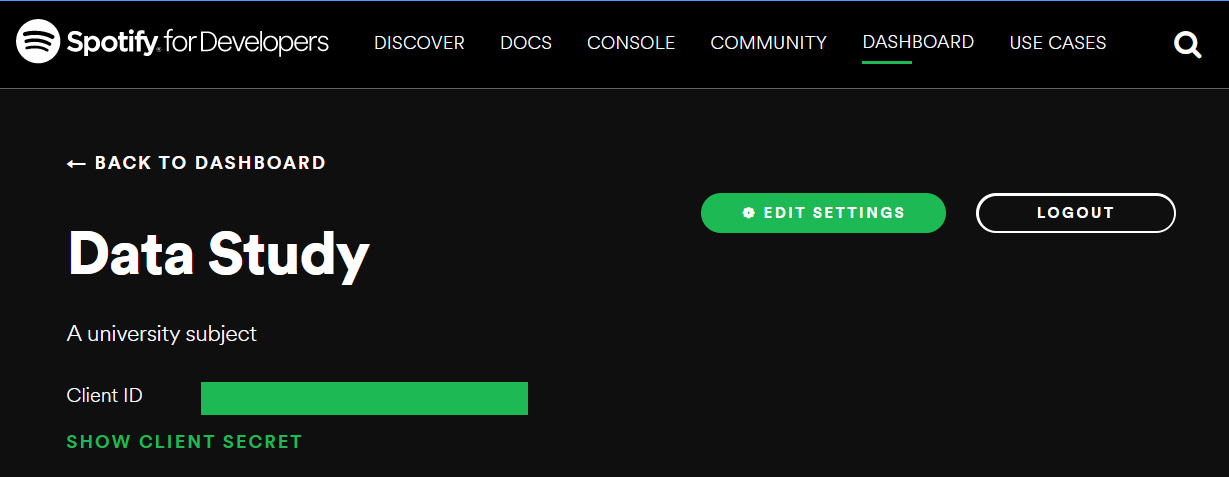
\includegraphics[width=120mm]{devoloper_spotify_1.png}
    \caption{Spotify application}\label{fig:app_spotify}
\end{figure}

\paragraph*{Una vez tengamos nuestra aplicacion creada necesitaremos el client ID y el client secret para poder autenticarnos 
y recuperar datos de la API.}

\paragraph*{Nuestro trabajo se compone de dos programas, el primero escrito en Python utilizando Visual Studio Code
que nos permite recuperar datos de la API de Spotify y exportarlos a JSON, y el segundo escrito en SageMath que nos permite representar y estudiar esos datos con Teoría de Grafos.}

\section{Obtención de datos}

\paragraph*{El codigo python se compone de tres secciones}
\begin{itemize}
	\item \textbf{Conexión}
	\item \textbf{Recolección de datos}
	\item \textbf{Exportación}
\end{itemize}

\paragraph*{Para que el codigo funcione solo se han necesitado 3 librerías:}
\begin{itemize}
	\item \textbf{spotipy.oauth2-SpotifyClientCredentials:} nos permite hacer la autenticación.
	\item \textbf{pandas:} nos permite crear los dataframes que vamos a exportar a SageMath.
	\item \textbf{spotipy:} nos permite interactuar con la API.
\end{itemize}
\paragraph*{A continuación se explicaran las imágenes presentes en la Figura~\ref{fig:codigoPython}.}


\paragraph*{Lo primero que hacemos es obtener todas las playlists relacionadas con el artista. Para ello hemos tomado la URL de cada una de las playlists de 50 Cent y las hemos almacenado para su posterior uso. 
Tras ello, para cada playlist llamamos al comando sp.user\textunderscore playlist, que nos permite obtener los datos de una playlist dada su URL, para más tarde almacenar las canciones que contiene cada una.}

\paragraph*{Una vez obtenidas las canciones, creamos un bucle con el que para cada canción que hayamos obtenido, obtenemos primeramente un dataset de las playlists, donde metemos los nombres de las canciones junto al nombre de sus artistas. 
Tras hacer eso, creamos un dataset con los artistas, obteniendo su nombre, géneros musicales asociados, popularidad y seguidores con el comando sp.artist. }

\paragraph*{Finalmente, convertimos los datasets obtenidos anteriormente en Data Frames usando pandas (en el código lo usamos como pd) que posteriormente son procesados en formato JSON con el comando .to\textunderscore json, al cual le pasamos como argumento la ubicación de donde va a terminar el fichero con los datos y el dataframe correspondiente. }

\pagebreak
\begin{figure}[H]
	\begin{center}
%
	   \subfigure[conexion API]{%
		   \label{fig:first}
		   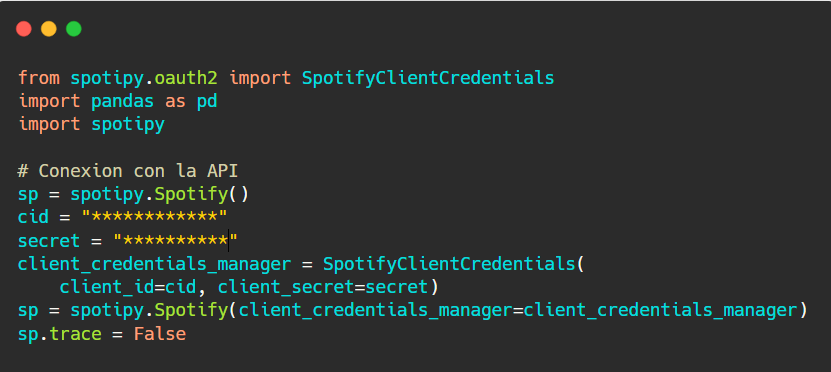
\includegraphics[width=0.7\textwidth]{programa_1.png}
	   }%
	   
	   \subfigure[Urls que utilizaremos con la API]{%
		   \label{fig:second}
		   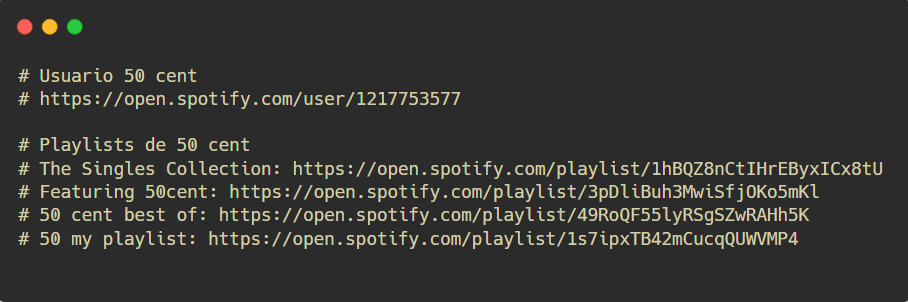
\includegraphics[width=0.7\textwidth]{programa_2.png}
	   }\\ %  ------- End of the first row ----------------------%
	   \subfigure[Recolección y exportación de los datos]{%
		   \label{fig:third}
		   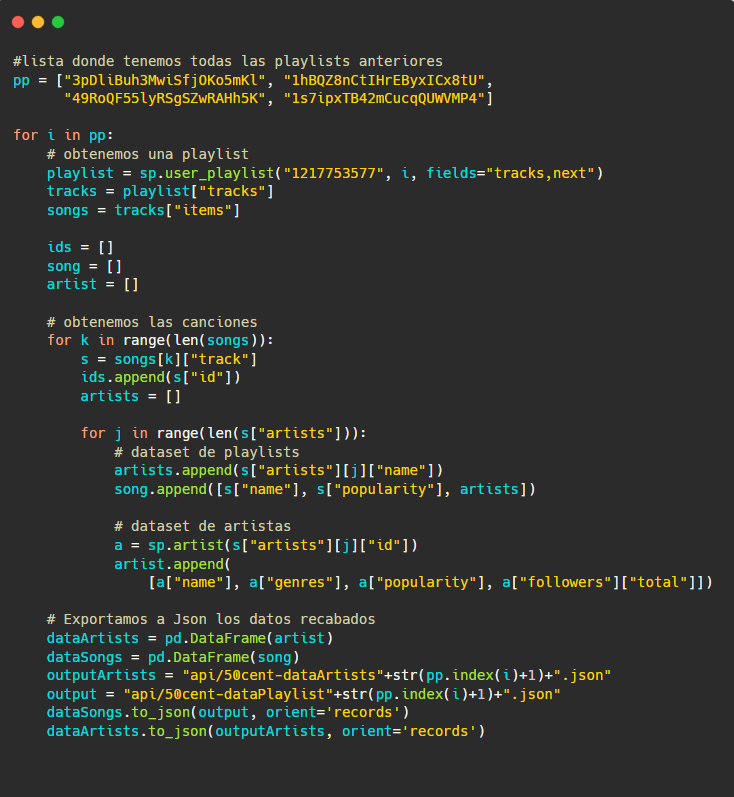
\includegraphics[width=0.7\textwidth]{programa_3.png}
	   }%
	  
%
	\end{center}
	\caption{%
	Código Python
 	}%
	\label{fig:codigoPython}
\end{figure}

\pagebreak

\section{Creación del grafo y otros cálculos}

\paragraph*{Una vez hemos extraído los datos de la API es turno de importar los datos JSON, para ello utilizaremos la librería \emph{json}.}

\paragraph*{Una vez importado utilizaremos dos listas que englobaran los 4 datasets, uno para las playlist y otro para los artistas.Figura~\ref{fig:codigoSage1}}

\paragraph*{Para crear el grafo hemos recorrido cada playlist y enlazado aquellos artistas que aparecen en dicha playlist, 
el resultado es un grafo en donde cada color representa una playlist y cada vértice un artista. Figura~\ref{fig:codigoSage2}.}



\begin{figure}[H]
	\begin{center}
%
	   \subfigure[librerias json]{%
		   \label{fig:first}
		   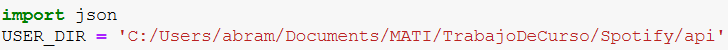
\includegraphics[width=0.7\textwidth]{sage_1.png}
	   }%
	   
	   \subfigure[importación de los datos de los artistas]{%
		   \label{fig:second}
		   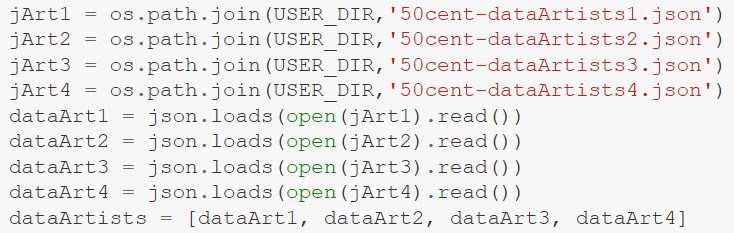
\includegraphics[width=0.7\textwidth]{sage_2.png}
	   }\\ %  ------- End of the first row ----------------------%
	   \subfigure[importación de los datos de las playlists]{%
		   \label{fig:third}
		   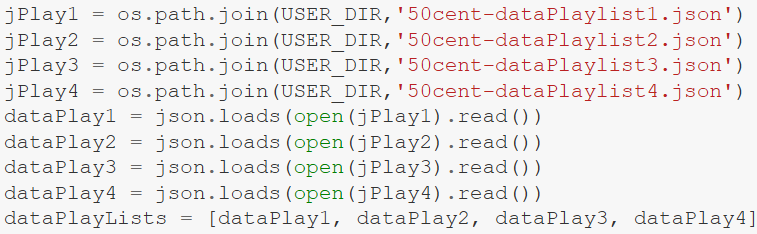
\includegraphics[width=0.7\textwidth]{sage_3.png}
	   }%
	  
%
	\end{center}
	\caption{%
	Código SageMath 1
 	}%
	\label{fig:codigoSage1}
\end{figure}

\begin{figure}[H]
	\begin{center}
%
	   \subfigure[metódos auxiliares para crear el grafo]{%
		   \label{fig:first}
		   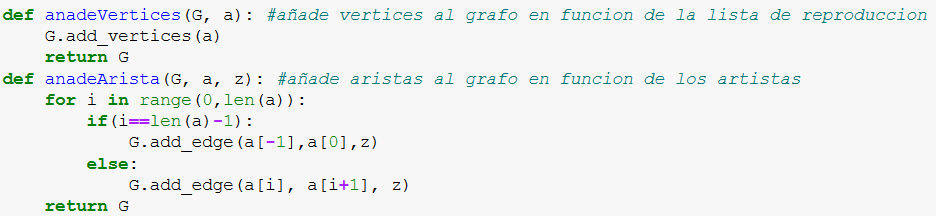
\includegraphics[width=0.7\textwidth]{sage_5.png}
	   }%
	   
	   \subfigure[creación del grafo]{%
		   \label{fig:second}
		   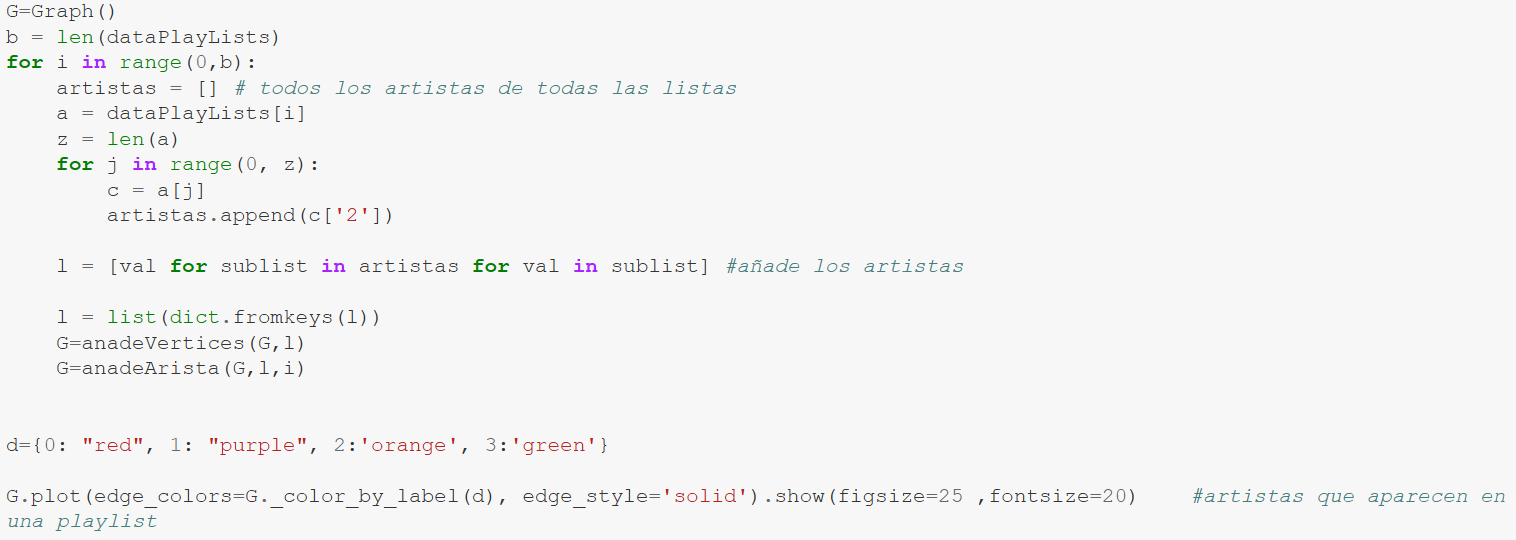
\includegraphics[width=0.7\textwidth]{sage_4.png}
	   }\\ %  ------- End of the first row ----------------------%
	   \subfigure[grafo]{%
		   \label{fig:third}
		   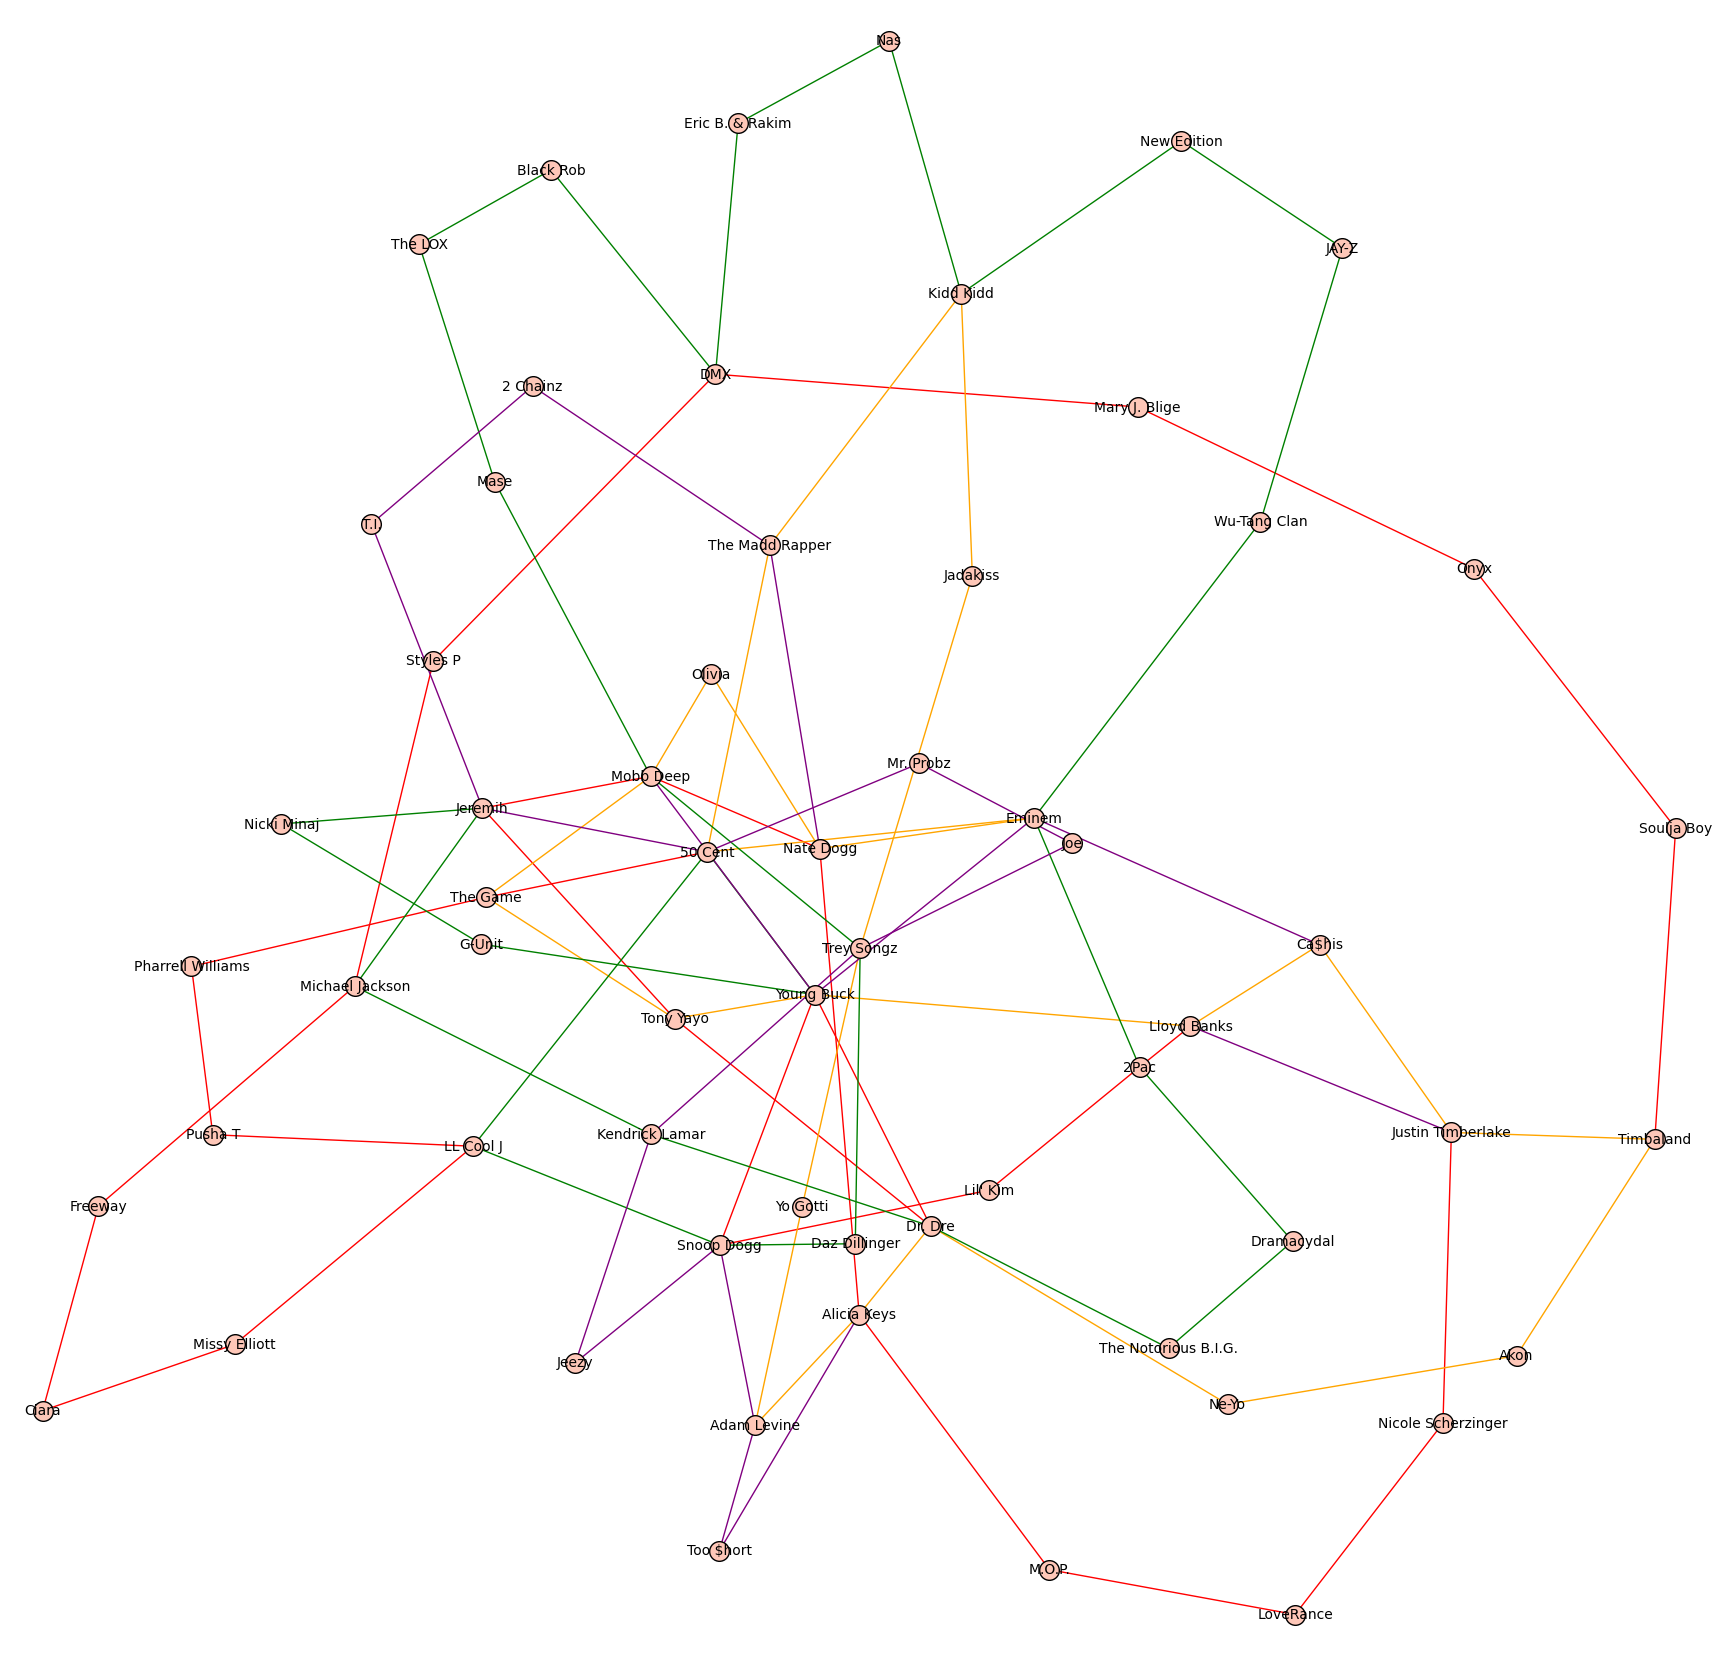
\includegraphics[width=0.7\textwidth]{sage_6.png}
	   }%
	  
%
	\end{center}
	\caption{%
	Código SageMath 2
 	}%
	\label{fig:codigoSage2}
\end{figure}


\paragraph*{De los artistas que participan en las playlists se han obtenido 
los más populares por cada playlists, del más popular se puede ver que Eminen es el ganador. Figura~\ref{fig:codigoSage3}.}

\paragraph*{Se pueden observar las comunidades segun los géneros por artista, 
de las playlist anteriores podemos encontrar que los generos raíz son el hiphop y el rap
y podemos ver géneros derivados como el nashville hip hop o el electropop. Figura~\ref{fig:codigoSage3}.}

\paragraph*{La centralidad de intermediacion nos permite detectar 
aquellos nodos que hacen de puente para otros nodos de tal forma que el camino se hace mas corto.
En este grafo tras aplicar la centralidad de intermediacion y coger los valores mas altos 
podemos observar que los mas importantes son Young Buck y 50 cent, 
curioso ya que 50 cent esta en todas las playlists. Figura~\ref{fig:codigoSage4}.}

\paragraph*{Prácticamente coincide con el centro del grafo(cercania) Figura~\ref{fig:codigoSage4}.}

\paragraph*{Lo sorpredente de esta centralidad de grado es que a pesar de que 50 Cent es nuestro 
autor de estudio Mobb Deep tiene la misma centralidad de grado. Figura~\ref{fig:codigoSage4}.}


\begin{figure}[H]
	\begin{center}
%
	   \subfigure[Popularidad total según playlist]{%
		   \label{fig:first}
		   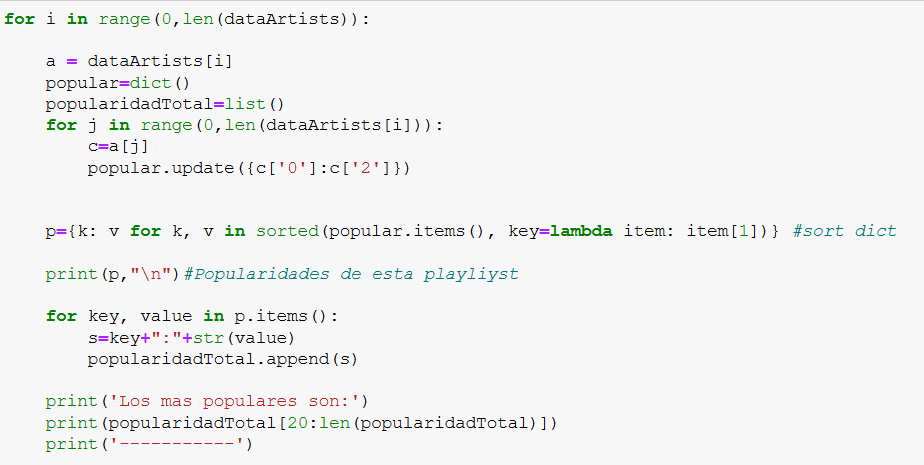
\includegraphics[width=0.5\textwidth]{sage_7.png}
	   }%
	   \subfigure[Salida popularidad total según playlist]{%
		   \label{fig:second}
		   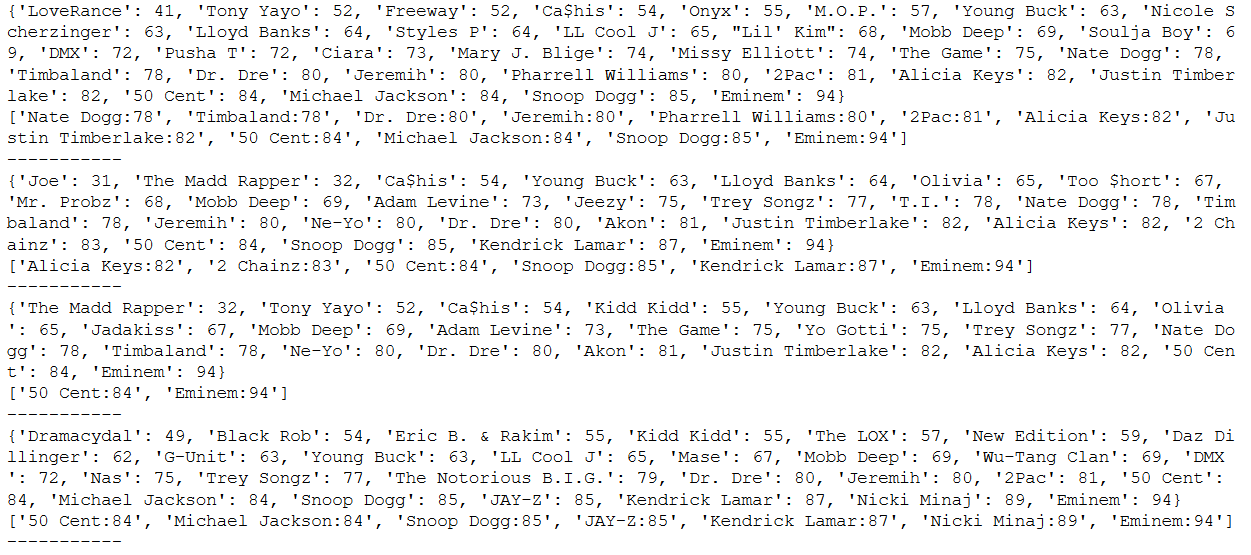
\includegraphics[width=0.5\textwidth]{sage_7_out.png}
	   }\\ %  ------- End of the first row ----------------------%
	   \subfigure[Género mas popular según playlist]{%
		   \label{fig:third}
		   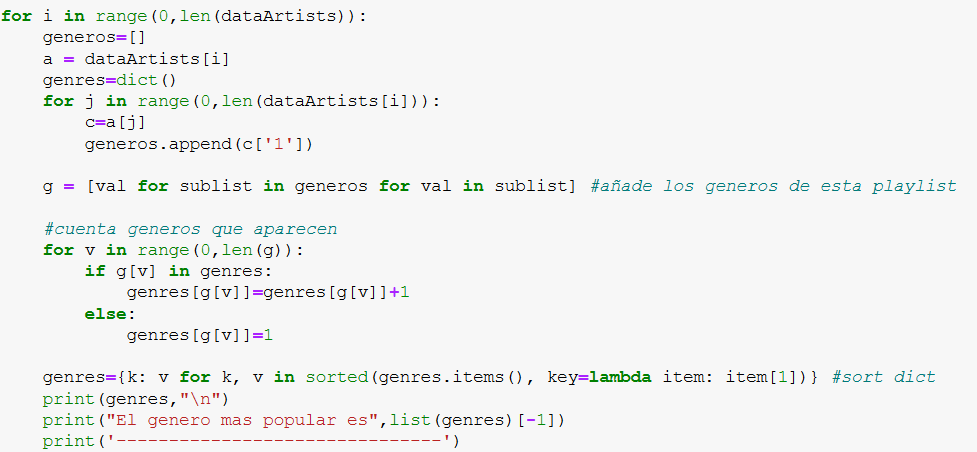
\includegraphics[width=0.5\textwidth]{sage_8.png}
	   }%
	   \subfigure[Salida Género mas popular según playlist]{%
		   \label{fig:four}
		   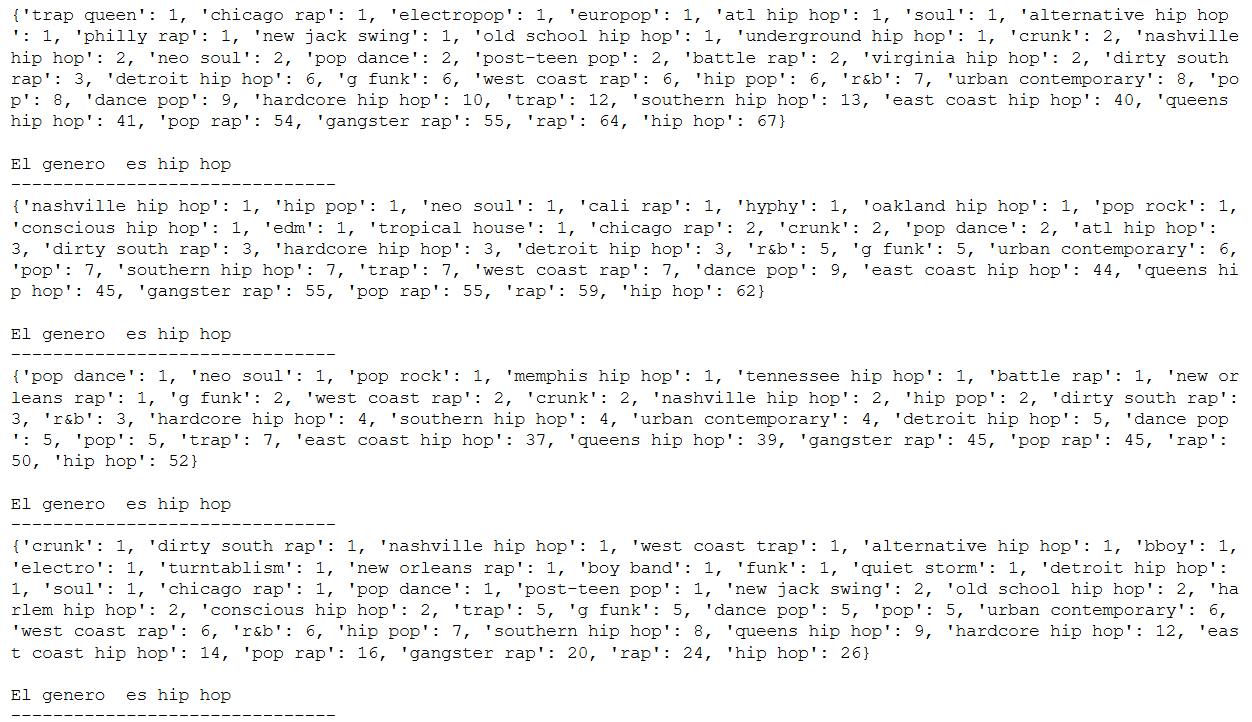
\includegraphics[width=0.5\textwidth]{sage_8_out.png}
	   }%
%
	\end{center}
	\caption{%
	Código SageMath 3
 	}%
	\label{fig:codigoSage3}
\end{figure}

\pagebreak

\begin{figure}[H]
	\begin{center}
%
	   \subfigure[Centralidad de grado]{%
		   \label{fig:first}
		   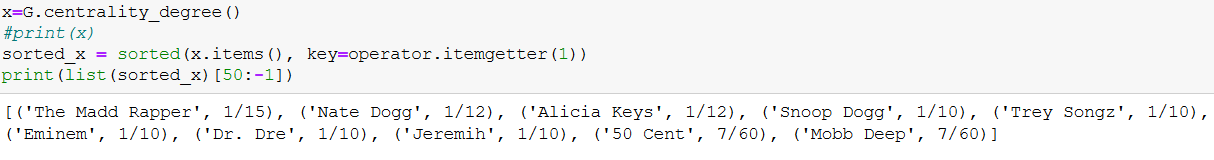
\includegraphics[width=1.0\textwidth]{sage_11.png}
	   }\\%  ------- End of the first row ----------------------%
	   \subfigure[Centralidad de intermediación]{%
		   \label{fig:second}
		   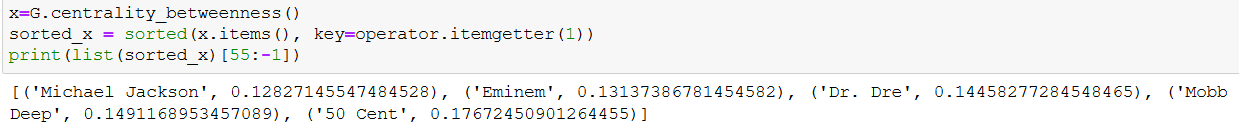
\includegraphics[width=1.0\textwidth]{sage_9.png}
	   }\\ %  ------- End of the first row ----------------------%
	   \subfigure[Centralidad de cercanía]{%
		   \label{fig:third}
		   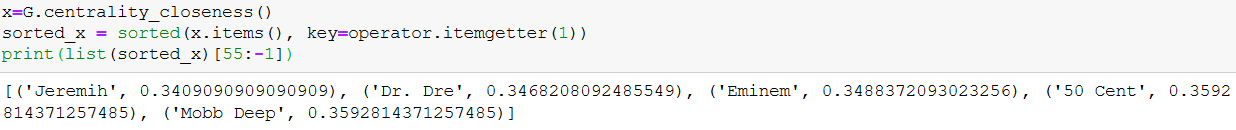
\includegraphics[width=1.0\textwidth]{sage_10.png}
	   }%
%
	\end{center}
	\caption{%
	Código SageMath 4
 	}%
	\label{fig:codigoSage4}
\end{figure}


\section{Estudio de comunidades}
\paragraph*{Para el estudio de comunidades utilizaremos la herramienta Gephi. 
Para ello es necesario tener los vértices y las aristas en formato CSV.
Esto se ha hecho a mano con un poco de paciencia, por ende es posible que haya alguna errata, 
aunque lo ideal es hacer algun tipo de algoritmo que dado un grafo de sage a partir de las listas de vertices y aristas,
haga la conversion a CSV y luego eso lo importaríamos en Gephi.}

\paragraph*{Una vez obtenidos los arhivos CSV el siguiente paso es importarlo en la herramienta, para ello seguiremos los siguientes pasos:}
\begin{enumerate}
	\item \textbf{Archivo, Importar hoja de cálculo.}
	\item \textbf{Seleccionamos el archivo CSV que contiene los vértices.}
	\item \textbf{Le damos siguiente, terminar y añadir a espacio de trabajo existente.}
	\item \textbf{Repetimos el proceso pero esta vez con el archivo de aristas}
	\item \textbf{Le damos siguiente a todo y no olvidemos al acabar de añadir las aristas al espacio de trabajo existente.}
\end{enumerate}

\paragraph*{A continuación en el panel de estadísticas ejecutaremos el algoritmo de Modularidad que nos dará las estadísticas. 
Podemos observar que se han detectado 7 comunidades, que para representarlas en el grafo y poder verlas visualmente tenemos que configurar los siguientes elementos: [Figura~\ref{fig:gephiModularity}].}
\begin{enumerate}
	\item \textbf{Apariencia(icono de la paleta de colores), Nodos, Partición y seleccionamos Modularity Class. De esta forma los nodos se colorearan del color correspondiente a su comunidad.}
	\item \textbf{Apariencia(icono del tamaño), Ranking, Betweenness Centrality. Para que el tamaño de los nodos represente la centralidad de cercanía..}
	\item \textbf{En Distribución, seleccionamos Force Atlas y ajustamos la fuerza de repulsión en 100000.0 y marcamos Ajustar por tamaños.}
	\item \textbf{Por último se han coloreado las aristas por peso para distinguir las playlists que los unen.}
	\item \textbf{Obtenemos el grafo de la figura. }
\end{enumerate}

\begin{figure}[H]
	\begin{center}
%
	   \subfigure[Resultado de la modularidad]{%
		   \label{fig:first}
		   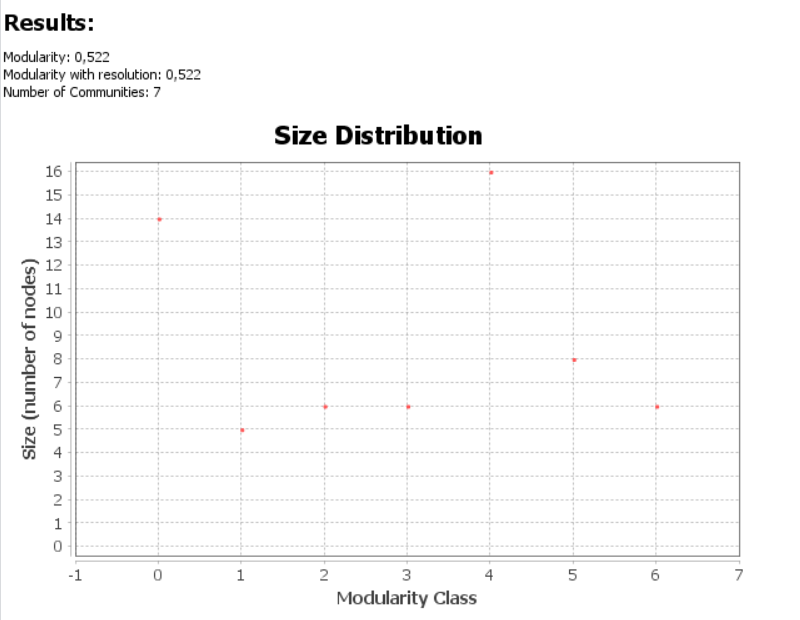
\includegraphics[width=0.5\textwidth]{gephi_modularity.png}
	   }%
	   \subfigure[Apariencia color nodos]{%
		   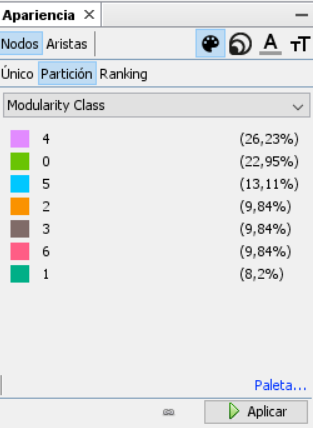
\includegraphics[width=0.3\textwidth]{gephi_apariencia_color.png}
		   \label{fig:second}
	   }\\ %  ------- End of the first row ----------------------%
	   \subfigure[Apariencia tamaño nodos]{%
		   \label{fig:third}
		   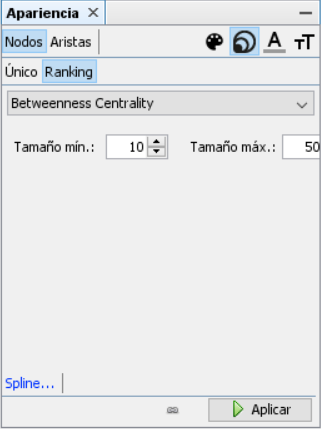
\includegraphics[width=0.3\textwidth]{gephi_apariencia_tam.png}
	   }%
	   \subfigure[Grafo por comunidades]{%
	   \label{fig:four}
	   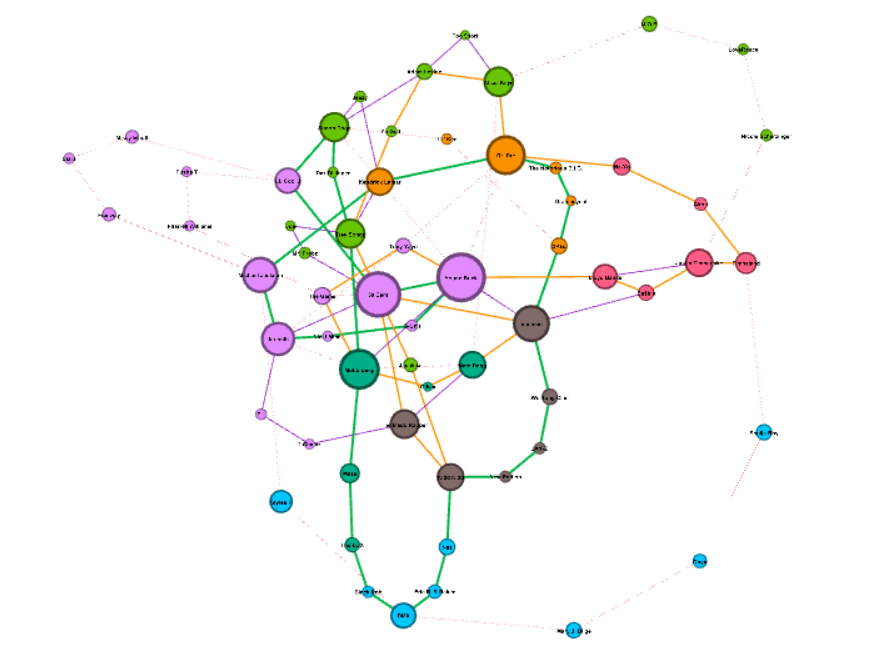
\includegraphics[width=0.5\textwidth]{gephi_graph_1.png}
   	   }%
%
	\end{center}
	\caption{%
	Modularidad en Gephi
 	}%
	\label{fig:gephiModularity}
\end{figure}

\paragraph*{Si utilizamos la pestaña de previsualización de Gephi obtendremos la Figura~\ref{fig:gephi_bonito} y podremos ver las 7 comunidades un poco más de cerca, 
dónde el tamaño de los nodos representan una centralidad de cercanía en la que cuanto mayor es el nodo mayor es su centralidad, que a su vez coincide con el ranking de popularidad de cada artista.}

\begin{figure}[h!]
    \centering
    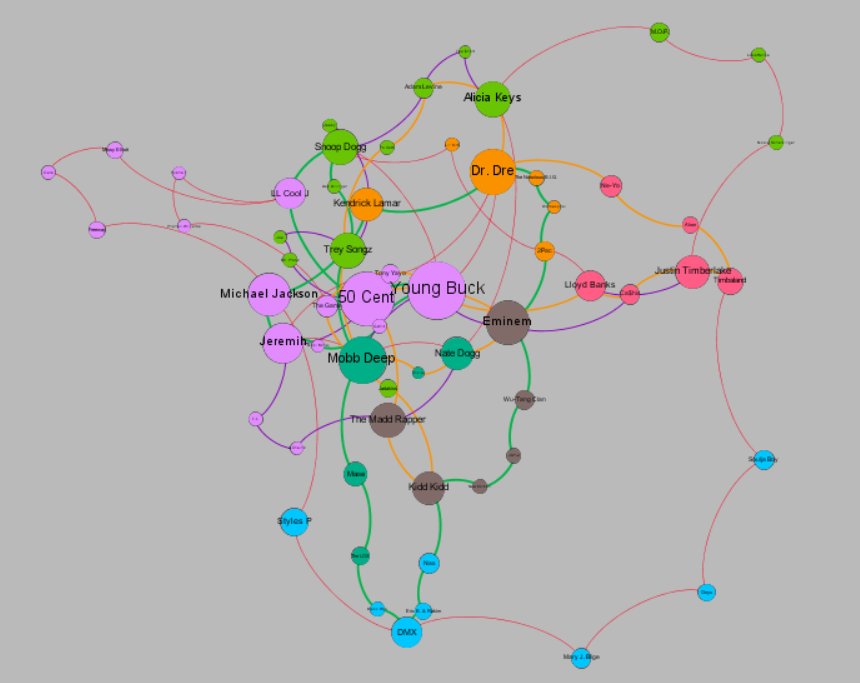
\includegraphics[width=150mm]{gephi_grafo_bonito.png}
    \caption{Gephi, grafo por comunidades}\label{fig:gephi_bonito}
\end{figure}
\pagebreak

\section{Conclusiones}

\paragraph*{A diferencia de otras redes como Twitter o Facebook, Spotify es un tanto más difícil de estudiar ya que no es tan susceptible de que un ojo novato cree con poco esfuerzo un boceto de como funcionan las relaciones entre artistas, 
no como en Facebook que con ir diciendo premisas como "Fulanito es amigo de Pepito, así que puedo unirlos con una arista, y entonces...", o "Naranjito le dio retweet a Manolito, así que puedo relacionarlos con una arista, y entonces...", obtener una red es asequible. Spotify te puede ofrecer en cambio listas de reproducción con ciertos artistas, álbumes de esos artistas e incluso podcasts, lo que hace que el ojo inexperto tenga problemas para buscar una forma de estudiar la red. }

\paragraph*{Sin embargo, al estudiar a un artista en concreto como 50 Cent a partir de sus listas de reproducción, hemos obtenidos resultados interesantes, como que por ejemplo él no sea el artista más famoso de su grupo, sino Eminem, o que por ejemplo un artista como Mobb Deep sea un artista de paso entre todas las listas de reproducción.
Todos estos resultados fueron gratificantes y cuanto menos informativos del comportamiento de Spotify.
\footnote{Todo el trabajo realizado se puede encontrar en \href{https://github.com/AbramsM1A2/Spotify}{GitHub}.}}

\section{Bibliografía}

\paragraph*{[Página web] Grafos y Sage, URL: \url{https://doc.sagemath.org/pdf/en/reference/graphs/graphs.pdf}.}

\paragraph*{[Página web] Perfil de 50 Cent, URL: \url{https://open.spotify.com/user/1217753577 }.}

\paragraph*{[Página web] Spotify Web API, URL: \url{https://developer.spotify.com/documentation/web-api/}.}

\paragraph*{[Página web] Referencia Spotify Web API, URL: \url{https://developer.spotify.com/documentation/web-api/reference-beta/}.}

\paragraph*{[Página web] Atributos de la API, URL: \url{https://developer.spotify.com/documentation/web-api/reference/tracks/get-track/}.}

\paragraph*{[Página web] Tutorial de la API de Spotify en español, URL: \url{http://gerardoprieto.com/2019/02/12/jugando-con-python-y-el-api-de-spotify/}.}



\end{document}
